\chapter{Organometaalchemie: binding en liganden}\label{ch:b3:organometallic-bonding}

In 1951 verkregen twee onderzoeksgroepen, onafhankelijk van elkaar, een
oranje, luchtstabiel poeder met de formule $\ce{FeC10H10}$ dat nergens op leek te slaan:
ijzer vormt gewoonlijk geen stabiele bindingen met koolstof, en zeker
niet met twee cyclopentadienylringen tegelijk. Binnen een jaar was de
structuur vastgesteld: het ijzer zit tussen twee evenwijdige ringen, even
sterk gebonden aan alle tien koolstofatomen, een sandwich. Ferroceen
opende de moderne organometaalchemie, waarvan de katalysatoren nu het
grootste deel van de polymeren, geneesmiddelen en fijnchemicaliën ter
wereld maken (\cref{ch:b3:homogeneous-catalysis}).
Dit hoofdstuk legt uit hoe metalen binden aan koolstofmonoxide,
fosfines, alkenen, ringen, \omterm{def:b3:organometallic-bonding:carbene}{carbenen} en aan elkaar, en hoe de \omterm{def:b3:organometallic-bonding:isolobal}{isolobale
analogie} organometaalfragmenten verbindt met de organische chemie van
koolstof.

\begin{recall}
Het deel van jaar~1 definieerde organometaalverbindingen en gebruikte
grignardreagentia.
Het deel van jaar~2 voerde de 18-elektronenregel en de
valentie-elektronentelling in, de hapticiteit, $\pi$-acceptorliganden en $\pi$-donorliganden met terugdonatie, de elementaire
stappen van organometaalreacties (oxidatieve additie, reductieve
eliminatie, insertie) en fragmentorbitalen.
\Cref{ch:b3:group-theory-applied} telde de IR-actieve CO-strekvibraties
van carbonylen en bouwde symmetrieaangepaste combinaties;
\cref{ch:b3:complex-spectra-magnetism} verbond magnetische momenten met
ongepaarde elektronen.
\end{recall}

\begin{omfigure}
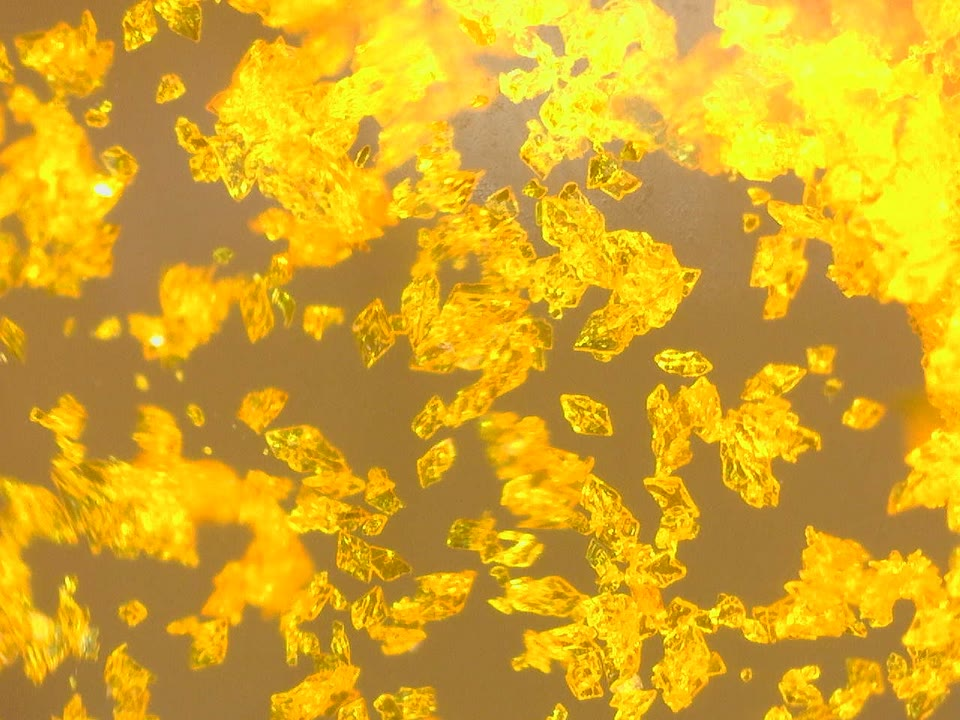
\includegraphics[width=0.5\linewidth]{images/book4/ferrocene-crystals.jpg}

{\small Kristallen van ferroceen, $\ce{Fe(C5H5)2}$: een oranje organometaalverbinding
die stabiel is aan de lucht en bij zacht verwarmen sublimeert.}
\end{omfigure}

\section{Elektronentelling en oxidatietoestanden}

\begin{method}[Elektronen tellen, op twee manieren]\label{met:b3:organometallic-bonding:count}
\begin{enumerate}
  \item Methode van de neutrale liganden (covalente methode): het metaal
        brengt zoveel elektronen mee als zijn groepsnummer; elk ligand,
        neutraal genomen, brengt er 1 (H, \ce{CH3}, Cl, het
        $\eta^1$-allyl) of 2 (CO, \ce{PR3}, alkeen) of meer ($\eta^5$-\ce{C5H5} 5, $\eta^6$-\ce{C6H6} 6); tel er één bij per
        metaal-metaalbinding en corrigeer voor de totale lading.
  \item Ionische methode: liganden zoals H, \ce{CH3}, Cl, \ce{C5H5} worden geteld als anionen (2, 2,
        2 en 6 elektronen), en het metaal als het kation $d^n$ dat daaruit volgt; neutrale liganden
        zoals voorheen.
  \item Beide geven hetzelfde totaal; de ionische methode geeft ook de
        oxidatietoestand
        en de $d^n$-configuratie.
\end{enumerate}
\end{method}

\begin{example}[Tellen]\label{ex:b3:organometallic-bonding:count}
$\ce{Fe(CO)5}$: $8 + 5 \times 2 = 18$, ijzer(0), $d^8$. Ferroceen: neutrale methode $8 + 2 \times 5 = 18$; ionische methode
$\ce{Fe^{2+}}$ ($d^6$, 6) $+ 2 \times 6$ ($\ce{C5H5-}$) $= 18$, ijzer(II). $\ce{Mn2(CO)10}$: elk Mn $7 + 5 \times 2 + 1$ (de binding Mn--Mn) $= 18$. Vlakke vierkante complexen $d^8$ zoals $\ce{[PtCl4]^{2-}}$ of de katalysator van Wilkinson
$\ce{RhCl(PPh3)3}$ hebben 16 elektronen: hun lege orbitaal van het type $p_z$ ligt te hoog om gevuld te worden, en
vlakke vierkante complexen met 16 elektronen zijn even stabiel als
complexen met 18.
\end{example}

\section{Carbonylen en fosfines}

\begin{definition}[Metaalcarbonylen]\label{def:b3:organometallic-bonding:carbonyl}
Een \emph{metaalcarbonyl}\index{metaalcarbonyl} is een complex met
koolstofmonoxide als ligand. Een
\emph{terminaal carbonyl}\index{terminaal carbonyl} is via het koolstofatoom
aan één metaal gebonden; een
\emph{overbruggend carbonyl}\index{overbruggend carbonyl} overspant
twee (of drie) metalen.
\end{definition}

Ludwig Mond ontdekte in 1890 dat nikkel bij gewone temperatuur met
koolstofmonoxide reageert tot de vluchtige vloeistof $\ce{Ni(CO)4}$, die bij verhitting weer uiteenvalt in zuiver
nikkel: de basis van een raffinageproces. Koolstofmonoxide bindt aan
overgangsmetalen via zijn hoogste bezette orbitaal, een vrij $\sigma$-elektronenpaar dat
vooral op het koolstofatoom zit, en neemt elektronen op in zijn lege $\pi^*$-orbitalen, die ook
groter zijn op het koolstofatoom.

\begin{definition}[Synergetische binding]\label{def:b3:organometallic-bonding:synergic}
\emph{Synergetische binding}\index{synergetische binding} is de wederzijdse
versterking van de
$\sigma$-donatie van een ligand naar een metaal en de $\pi$-terugdonatie van het metaal naar het
ligand: de donatie maakt het metaal rijker aan elektronen en meer
geneigd ze terug te geven, de terugdonatie neemt de lading weg die door
de donatie opgebouwd is.
\end{definition}

\begin{omfigure}
\begin{tikzpicture}[font=\small, >=Stealth]
  % sigma donation
  \fill[black!70] (0,0) circle (0.14); \node[anchor=north] at (0,-0.4) {M};
  \pic at (0,0) {omlobe={-0.7}{180}};
  \pic at (0,0) {omlobe={0.9}{0}};
  \node[circle, fill=black!40, inner sep=1.6pt] at (1.9,0) {};
  \node[circle, fill=omThm!70, inner sep=1.6pt] at (3.0,0) {};
  \pic at (1.9,0) {omlobe={0.85}{180}};
  \node[font=\scriptsize, anchor=north] at (1.9,-0.25) {C};
  \node[font=\scriptsize, anchor=north] at (3.0,-0.25) {O};
  \draw[->, thick, omThm] (1.4,0.55) to[bend right=30] (0.6,0.55);
  \node[anchor=north] at (1.5,-1.55) {$\sigma$-donatie};
  % pi back-donation
  \begin{scope}[xshift=6.0cm]
    \fill[black!70] (0,0) circle (0.14); \node[anchor=north] at (0,-1.1) {M};
    \pic at (0,0) {omdxz};
    \node[circle, fill=black!40, inner sep=1.6pt] at (1.9,0) {};
    \node[circle, fill=omThm!70, inner sep=1.6pt] at (3.0,0) {};
    \pic at (1.9,0) {omp={0.9}{90}};
    \pic at (3.0,0) {omp={-0.6}{90}};
    \draw[->, thick, omThm] (0.6,1.05) to[bend left=30] (1.6,1.05);
    \node[anchor=north] at (1.5,-1.55) {$\pi$-terugdonatie};
  \end{scope}
\end{tikzpicture}

{\small \omterm{def:b3:organometallic-bonding:synergic}{Synergetische binding} van koolstofmonoxide. Links: het vrije
elektronenpaar van het koolstofatoom ($\sigma$-orbitaal)
doneert in een lege metaalorbitaal van het type $\sigma$. Rechts: een gevulde $d$-orbitaal van het metaal
($d_{xz}$, met haar twee assen) overlapt met de lege $\pi^*$-orbitaal van CO, die groter is op het
koolstofatoom en waarvan de lobben in fase passen: elektronen stromen
terug in een orbitaal die
antibindend is tussen C en O.}
\end{omfigure}

\begin{proposition}[CO-strekfrequenties]\label{prop:b3:organometallic-bonding:co-frequency}
Hoe meer een metaal terugdoneert in de $\pi^*$-orbitalen van een CO-ligand, hoe lager het
golfgetal van de strekvibratie C--O.
\end{proposition}

\begin{proof}[Beargumenteerd]
De $\pi^*$-orbitalen van CO zijn antibindend tussen C en O: ze bezetten verzwakt de
binding C--O, verlaagt haar \omterm{def:b3:quantum-model-systems:oscillator}{krachtconstante} en dus het golfgetal van de
strekvibratie, dat varieert als de vierkantswortel van de \omterm{def:b3:quantum-model-systems:oscillator}{krachtconstante} (\cref{ch:b3:rovibrational-spectroscopy}).
$\sigma$-donatie onttrekt elektronen aan een orbitaal die voor C--O
nagenoeg niet-bindend (licht antibindend) is, wat op zich het golfgetal
een beetje zou verhogen: de waargenomen daling toont dat de terugdonatie
overheerst.
\end{proof}

Vrij koolstofmonoxide heeft zijn \omterm{def:b3:rovibrational-spectroscopy:anharmonic}{fundamentele overgang} bij $\omega_e - 2\omega_ex_e = \qty{2143}{cm^{-1}}$; terminale
carbonylen van neutrale complexen absorberen ruwweg tussen 1900 en \qty{2100}{cm^{-1}},
overbruggende carbonylen nog lager. Langs een iso-elektronische reeks
absorbeert een anionisch carbonyl bij een lager golfgetal dan het
neutrale, een kationisch bij een hoger: hoe elektronenrijker het metaal,
hoe meer het terugdoneert. Het aantal banden, uit de symmetrie
(\cref{ch:b3:group-theory-applied}), geeft de geometrie.
% ledger: diat:CO.we, diat:CO.wexe

\begin{proposition}[$\pi$-interacties en de ligandveldsplitsing]\label{prop:b3:organometallic-bonding:pi-delta}
In een octaëdrisch complex verhogen $\pi$-acceptorliganden $\Delta_{\mathrm o}$ en verlagen $\pi$-donorliganden
haar.
\end{proposition}

\begin{proof}
De $e_g$-orbitalen hebben alleen $\sigma$-symmetrie. De $t_{2g}$-orbitalen ($d_{xy}$, $d_{xz}$, $d_{yz}$) passen bij een combinatie $t_{2g}$
van $\pi$-orbitalen van de liganden: voor $d_{xy}$ biedt elk van de vier liganden in het vlak $xy$ een
$\pi$-orbitaal aan die loodrecht staat op zijn as M--L in dat vlak, en de
combinatie met afwisselende tekens heeft de symmetrie van $d_{xy}$ (de overige
combinaties transformeren als $t_{1g}$, $t_{1u}$ en $t_{2u}$ en vinden geen partner $d$). Twee orbitalen met
dezelfde symmetrie mengen en stoten elkaar af: de onderste wordt
omlaaggeduwd, de bovenste omhoog. Een
$\pi$-acceptor biedt lege orbitalen aan boven de verzameling $t_{2g}$, die omlaaggeduwd wordt: $\Delta_{\mathrm o}$
neemt toe. Een $\pi$-donor biedt gevulde orbitalen aan eronder, die haar omhoogduwen: $\Delta_{\mathrm o}$
neemt af. Het $e_g$-niveau blijft in beide gevallen onaangetast.
\end{proof}

Daarom staan CO en \ce{CN-} aan het sterke uiteinde van de spectrochemische reeks, en
halogeniden en hydroxide aan het zwakke uiteinde, zoals het deel van
jaar~2 vermeldde.

\begin{definition}[Parameters van Tolman]\label{def:b3:organometallic-bonding:tolman}
De \emph{kegelhoek van Tolman}\index{kegelhoek van Tolman} van een fosfine
is de tophoek van de kegel, gecentreerd op het metaal op een
standaardafstand, die de vanderwaalsoppervlakken van zijn substituenten
net omsluit: een maat voor zijn grootte.
De \emph{elektronische parameter van Tolman}\index{elektronische parameter van Tolman}
is het golfgetal van de symmetrische CO-strekvibratie van $\ce{Ni(CO)3L}$: hoe sterker het
fosfine L doneert, hoe lager het is.
\end{definition}

Fosfines worden via hun substituenten onafhankelijk afgestemd in grootte
en elektronendonatie: trialkylfosfines zijn sterkere donoren dan
triarylfosfines, fosfieten de zwakste; $\ce{P(tBu)3}$ is veel omvangrijker dan $\ce{PMe3}$. Omvangrijke fosfines begunstigen
lage coördinatiegetallen en een snelle dissociatie van liganden, wat
verklaart waarom ze in zoveel katalysatoren voorkomen.

\section{$\pi$-liganden}

\begin{definition}[Model van Dewar-Chatt-Duncanson]\label{def:b3:organometallic-bonding:dcd}
Het \emph{model van Dewar-Chatt-Duncanson}\index{model van Dewar-Chatt-Duncanson} van
de binding van een alkeen aan een metaal combineert de $\sigma$-donatie vanuit de $\pi$-orbitaal van C=C
naar een lege metaalorbitaal met de terugdonatie vanuit een gevulde $d$-orbitaal van het metaal in
de $\pi^*$-orbitaal van C=C. De limiet van sterke terugdonatie is een
\emph{metallacyclopropaan}\index{metallacyclopropaan}, een drieledige ring
met twee $\sigma$-bindingen M--C en een enkelvoudige binding C--C.
\end{definition}

\begin{proposition}[Gevolgen van de terugdonatie naar een alkeen]\label{prop:b3:organometallic-bonding:dcd}
Coördinatie verlengt de binding C=C en buigt de substituenten naar
achteren, weg van het metaal, des te meer naarmate de terugdonatie
toeneemt.
\end{proposition}

\begin{proof}[Beargumenteerd]
Elektronen wegnemen uit de (bindende) $\pi$-orbitaal en ze toevoegen aan de (antibindende) $\pi^*$-orbitaal
verlagen allebei de bindingsorde C--C. Het bijmengen van $\pi^*$-karakter
herhybridiseert de koolstofatomen in de richting van $sp^3$, waarvan de bindingen naar de substituenten
van het metaal weg wijzen, naar de geometrie van het \omterm{def:b3:organometallic-bonding:dcd}{metallacyclopropaan}.
\end{proof}

\begin{omfigure}
\begin{tikzpicture}[font=\small, >=Stealth]
  \fill[black!70] (0,0) circle (0.14); \node[anchor=north] at (0,-1.1) {M};
  \pic at (0,0) {omlobe={0.9}{0}};
  \foreach \y in {0.45,-0.45}{\node[circle, fill=black!40, inner sep=1.6pt] at (1.9,\y) {};}
  \pic at (1.9,0.45) {omp={-0.75}{0}};
  \pic at (1.9,-0.45) {omp={-0.75}{0}};
  \draw[->, thick, omThm] (1.3,1.0) to[bend right=30] (0.5,0.6);
  \node[anchor=north] at (1.2,-1.4) {$\sigma$: $\pi$(C=C) $\to$ M};
  \begin{scope}[xshift=5.6cm]
    \fill[black!70] (0,0) circle (0.14); \node[anchor=north] at (0,-1.1) {M};
    \pic at (0,0) {omdxy};
    \foreach \y in {0.45,-0.45}{\node[circle, fill=black!40, inner sep=1.6pt] at (1.9,\y) {};}
    \pic at (1.9,0.45) {omp={-0.75}{0}};
    \pic at (1.9,-0.45) {omp={0.75}{0}};
    \draw[->, thick, omThm] (0.7,0.9) to[bend left=30] (1.5,0.9);
    \node[anchor=north] at (1.2,-1.4) {$\pi$: M $\to$ $\pi^*$(C=C)};
  \end{scope}
\end{tikzpicture}

{\small Het \omterm{def:b3:organometallic-bonding:dcd}{model van Dewar-Chatt-Duncanson} van een zijdelings gebonden
alkeen (C=C
verticaal, het metaal links). Links: de gevulde $\pi$-orbitaal (twee $p$-orbitalen in
fase) doneert in een lege metaalorbitaal. Rechts: een gevulde $d$-orbitaal van het metaal
met passende fasen doneert in de lege $\pi^*$-orbitaal (de twee $p$-orbitalen in
tegenfase).}
\end{omfigure}

Het zout van Zeise, $\ce{K[PtCl3(C2H4)]}$, gemaakt in 1827, was de eerste organometaalverbinding
van een overgangsmetaal; zijn etheen staat loodrecht op het vlak \ce{PtCl3}, zoals
het model voorspelt. Allyl ($\eta^3$), diënen ($\eta^4$), arenen ($\eta^6$) en de cyclopentadienylring ($\eta^5$) binden op dezelfde manier via meerdere koolstofatomen tegelijk.

\begin{definition}[Metallocenen]\label{def:b3:organometallic-bonding:metallocene}
Een \emph{sandwichverbinding}\index{sandwichverbinding} heeft een metaal
tussen twee evenwijdige vlakke ringliganden die via al hun
koolstofatomen gebonden zijn; een
\emph{metalloceen}\index{metalloceen} is een sandwichverbinding met twee ringen $\eta^5$-cyclopentadienyl,
$\ce{M(C5H5)2}$.
\end{definition}

\begin{proposition}[De grensorbitalen van ferroceen]\label{prop:b3:organometallic-bonding:ferrocene}
In een \omterm{def:b3:organometallic-bonding:metallocene}{metalloceen} met evenwijdige ringen ($D_{5d}$) splitsen de $d$-orbitalen van het metaal op in $e_{2g}$
($d_{xy}$, $d_{x^2-y^2}$) en $a_{1g}$ ($d_{z^2}$), nagenoeg niet-bindend en dicht bij elkaar, en $e_{1g}^\ast$ ($d_{xz}$,
$d_{yz}$), sterk antibindend; ferroceen, met zes $d$-elektronen in $e_{2g}^4a_{1g}^2$, heeft 18
elektronen en geen ongepaard elektron.
\end{proposition}

\begin{proof}[Beargumenteerd]
De $\pi$-orbitalen van de twee ringen combineren tot symmetrieaangepaste paren $a_{1g}$, $a_{2u}$,
$e_{1g}$, $e_{1u}$, $e_{2g}$, $e_{2u}$ (uit de vijf $\pi$-orbitalen van elke ring, met nul, één en twee
knoopvlakken door de as). De gevulde combinatie $e_{1g}$ van de ringen overlapt
sterk met $d_{xz}$, $d_{yz}$ (elk één knoopvlak door de as): ze vormen bindende
orbitalen, vooral op de ringen, en antibindende $e_{1g}^\ast$, vooral op het metaal, die hoog liggen. $d_{xy}$, $d_{x^2-y^2}$
(twee knoopvlakken) ontmoeten alleen de lege $e_{2g}$-orbitalen van de ringen en worden door
terugdonatie licht gestabiliseerd; $d_{z^2}$ wijst naar het gat in het midden van elke ring en
overlapt nauwelijks. Zes elektronen vullen $e_{2g}$ en $a_{1g}$; met de twaalf elektronen van de
bindende ringcombinaties komt de telling op 18.
\end{proof}

\begin{omfigure}
\begin{tikzpicture}[font=\small]
  % sandwich drawing
  \begin{scope}[xshift=-1.0cm]
    \draw[thick, fill=black!8] (0,1.0) ellipse (1.0 and 0.3);
    \draw[thick, fill=black!8] (0,-1.0) ellipse (1.0 and 0.3);
    \foreach \a in {90,162,234,306,18}{\fill[black!60] ({cos(\a)},{1.0+0.3*sin(\a)}) circle (0.07);
      \fill[black!60] ({cos(\a)},{-1.0+0.3*sin(\a)}) circle (0.07);}
    \shade[ball color=orange!70!brown] (0,0) circle (0.2);
    \node[anchor=west] at (0.25,0) {Fe};
  \end{scope}
  % level diagram for four metallocenes
  \pic[transform shape] at (2.1,-0.9) {omlevel={u}{0.5}};
  \pic[transform shape] at (2.7,-0.9) {omlevel={ud}{0.5}};
  \pic[transform shape] at (2.4,-0.4) {omlevel={ud}{0.5}};
  \pic[transform shape] at (2.1,1.0) {omlevel={}{0.5}};
  \pic[transform shape] at (2.7,1.0) {omlevel={}{0.5}};
  \node[anchor=north] at (2.4,-1.3) {\ce{[FeCp2]+}};
  \node[anchor=north, font=\scriptsize] at (2.4,-1.75) {17 e$^-$};
  \pic[transform shape] at (4.3,-0.9) {omlevel={ud}{0.5}};
  \pic[transform shape] at (4.9,-0.9) {omlevel={ud}{0.5}};
  \pic[transform shape] at (4.6,-0.4) {omlevel={ud}{0.5}};
  \pic[transform shape] at (4.3,1.0) {omlevel={}{0.5}};
  \pic[transform shape] at (4.9,1.0) {omlevel={}{0.5}};
  \node[anchor=north] at (4.6,-1.3) {\ce{FeCp2}};
  \node[anchor=north, font=\scriptsize] at (4.6,-1.75) {18 e$^-$};
  \pic[transform shape] at (6.5,-0.9) {omlevel={ud}{0.5}};
  \pic[transform shape] at (7.1,-0.9) {omlevel={ud}{0.5}};
  \pic[transform shape] at (6.8,-0.4) {omlevel={ud}{0.5}};
  \pic[transform shape] at (6.5,1.0) {omlevel={u}{0.5}};
  \pic[transform shape] at (7.1,1.0) {omlevel={}{0.5}};
  \node[anchor=north] at (6.8,-1.3) {\ce{CoCp2}};
  \node[anchor=north, font=\scriptsize] at (6.8,-1.75) {19 e$^-$};
  \pic[transform shape] at (8.7,-0.9) {omlevel={ud}{0.5}};
  \pic[transform shape] at (9.3,-0.9) {omlevel={ud}{0.5}};
  \pic[transform shape] at (9.0,-0.4) {omlevel={ud}{0.5}};
  \pic[transform shape] at (8.7,1.0) {omlevel={u}{0.5}};
  \pic[transform shape] at (9.3,1.0) {omlevel={u}{0.5}};
  \node[anchor=north] at (9.0,-1.3) {\ce{NiCp2}};
  \node[anchor=north, font=\scriptsize] at (9.0,-1.75) {20 e$^-$};
  \node[anchor=east, font=\scriptsize] at (1.8,-0.9) {$e_{2g}$};
  \node[anchor=east, font=\scriptsize] at (1.8,-0.4) {$a_{1g}$};
  \node[anchor=east, font=\scriptsize] at (1.8,1.0) {$e_{1g}^\ast$};
\end{tikzpicture}

{\small Links: de sandwichstructuur van ferroceen (ringen in eclipsstand).
Rechts: de
grensorbitalen van metallocenen met $d$-karakter: $e_{2g}$ en $a_{1g}$ nagenoeg niet-bindend, $e_{1g}^\ast$
antibindend, gevuld voor het ferroceniumkation (17 elektronen), ferroceen
(18), cobaltoceen (19) en nikkeloceen (20, één elektron in elke $e_{1g}^\ast$-orbitaal, spins
parallel volgens de regel van Hund).}
\end{omfigure}

\section{Carbenen, carbynen en metaal-metaalbindingen}

\begin{definition}[Carbenen en carbeencomplexen]\label{def:b3:organometallic-bonding:carbene}
Een \emph{carbeen}\index{carbeen} is een neutraal deeltje $\ce{R2C}$ met een tweewaardig koolstofatoom
dat twee niet-bindende elektronen draagt. Een
\emph{carbeencomplex}\index{carbeencomplex}
heeft een ligand $\ce{CR2}$ dat met een dubbele binding aan een metaal gebonden is, $\ce{M=CR2}$. Een
complex met een \emph{fischercarbeen}\index{fischercarbeen} heeft een
heteroatoomsubstituent op het carbeenkoolstofatoom en een laagvalent
metaal met $\pi$-acceptorliganden; zijn carbeenkoolstofatoom
is elektrofiel. Een complex met een
\emph{schrockcarbeen}\index{schrockcarbeen} (alkylideen)
heeft alleen substituenten C of H en een hoogvalent vroeg metaal; zijn
koolstofatoom is nucleofiel. Een
\emph{N-heterocyclisch carbeen}\index{N-heterocyclisch carbeen} is een
cyclisch carbeen geflankeerd door twee stikstofatomen, stabiel als vrije
verbinding en een sterk
$\sigma$-donorligand.
\end{definition}

De twee soorten \omterm{def:b3:organometallic-bonding:carbene}{carbeencomplexen} verschillen in de manier waarop de
binding M=C gedeeld wordt.
In een \omterm{def:b3:organometallic-bonding:carbene}{fischercarbeen} doneert een singuletcarbeen zijn vrije
elektronenpaar aan het metaal en ontvangt het terugdonatie in zijn lege $p$-orbitaal, die het vrije
elektronenpaar van het heteroatoom ook stabiliseert: het koolstofatoom
blijft elektronenarm en wordt door nucleofielen aangevallen. In een
\omterm{def:b3:organometallic-bonding:carbene}{schrockcarbeen} vormen twee tripletfragmenten, metaal en \omterm{def:b3:organometallic-bonding:carbene}{carbeen}, een covalente binding $\sigma +
\pi$, gepolariseerd naar het koolstofatoom: het alkylideen gedraagt zich als een wittigylide.

\begin{definition}[Carbyncomplex]\label{def:b3:organometallic-bonding:carbyne}
Een \emph{carbyncomplex}\index{carbyncomplex} heeft een drievoudige binding
tussen een metaal en een koolstofatoom met één substituent, $\ce{M#CR}$.
\end{definition}

\begin{definition}[$\delta$-binding, viervoudige binding]\label{def:b3:organometallic-bonding:delta}
Een \emph{$\delta$-binding}\index{delta-binding@$\delta$-binding} is een binding waarvan de orbitaal twee knoopvlakken heeft
die de internucleaire as bevatten, gevormd door de overlap van aangezicht
tot aangezicht van twee $d$-orbitalen zoals $d_{xy}$ en $d_{xy}$. Een
\emph{viervoudige binding}\index{viervoudige binding}
combineert één $\sigma$-binding, twee $\pi$-bindingen en één $\delta$-binding tussen twee metaalatomen.
\end{definition}

\begin{proposition}[{De \omterm{def:b3:organometallic-bonding:delta}{viervoudige binding} van $[\mathrm{Re_2Cl_8}]^{2-}$}]\label{prop:b3:organometallic-bonding:quadruple}
In $\ce{[Re2Cl8]^{2-}}$ (twee \ce{Re^{III}}, elk $d^4$) bezetten de acht $d$-elektronen $\sigma^2\pi^4\delta^2$: een
bindingsorde 4, die de eclipsstand van de twee eenheden \ce{ReCl4} vereist.
\end{proposition}

\begin{proof}
Met $z$ langs de as Re--Re en de Cl-atomen langs $\pm x$ en $\pm y$ op elk Re wijst $d_{x^2-y^2}$
naar de chloriden en wordt ze gebruikt in de bindingen Re--Cl. De vier andere $d$-orbitalen
van elk metaal overlappen paarsgewijs: $d_{z^2}$ met $d_{z^2}$ langs de as ($\sigma$), $d_{xz}$ met $d_{xz}$ en $d_{yz}$
met $d_{yz}$ zij aan zij ($\pi$, tweemaal), $d_{xy}$ met $d_{xy}$ van aangezicht tot aangezicht ($\delta$, de zwakste).
Acht elektronen vullen de vier bindende combinaties. Een eenheid over $45^\circ$
draaien om $z$ maakt van haar $d_{xy}$ een $d_{x^2-y^2}$, die om symmetrieredenen nul overlap heeft met de andere $d_{xy}$:
de $\delta$-binding, en daarmee de voorkeur voor de eclipsstand, gaat
verloren. De andere drie overlappen zijn cilindersymmetrisch of
ongewijzigd in grootte.
\end{proof}

% ledger: geom:Re2Cl8.ReRe
De afstand Re--Re van \qty{2.24}{\angstrom} in het kaliumzout is zeer kort voor twee metaalatomen, en de chloriden van de twee helften staan inderdaad in eclipsstand, tegen
hun sterische afstoting in: de $\delta$-binding, hoe zwak ook, houdt ze daar.

\begin{omfigure}
\tdplotsetmaincoords{58}{25}
\begin{tikzpicture}[tdplot_main_coords, font=\small, scale=1.15]
  \draw[thick, black!60] (0,0,0) -- (0,0,2.0);
  \foreach \z in {0,2.0}{
    \foreach \b in {0,90,180,270}{
      \draw[black!45] (0,0,\z) -- ({1.55*cos(\b)},{1.55*sin(\b)},\z);}
    \foreach \a/\s in {45/omphasepos, 135/omphaseneg, 225/omphasepos, 315/omphaseneg}{
      \path[\s, opacity=0.9] plot[domain=0:360, samples=48, smooth cycle]
        ({0.62*cos(\a)+0.55*cos(\x)*cos(\a)-0.26*sin(\x)*sin(\a)},
         {0.62*sin(\a)+0.55*cos(\x)*sin(\a)+0.26*sin(\x)*cos(\a)}, {\z});}
    \foreach \b in {0,90,180,270}{
      \node[circle, fill=green!45!black, inner sep=1.8pt] at ({1.55*cos(\b)},{1.55*sin(\b)},\z) {};}
    \shade[ball color=black!40] (0,0,\z) circle (0.14);}
  \node[anchor=east, xshift=-1.9cm] at (0,0,2.0) {Re};
  \node[anchor=east, xshift=-1.9cm] at (0,0,0) {Re};
\end{tikzpicture}

{\small De $\delta$-component van de \omterm{def:b3:organometallic-bonding:delta}{viervoudige binding} van $\ce{[Re2Cl8]^{2-}}$: de $d_{xy}$-orbitalen van
de twee reniumatomen (elk vier lobben, tekens blauw en oranje) staan
tegenover elkaar over de as Re--Re, lob boven lob van hetzelfde teken. De chloriden (groen),
in eclipsstand, liggen langs $x$ en $y$, tussen de lobben.}
\end{omfigure}

\section{De isolobale analogie}

\begin{definition}[Isolobale fragmenten]\label{def:b3:organometallic-bonding:isolobal}
Twee moleculaire fragmenten zijn
\emph{isolobaal}\index{isolobale fragmenten} wanneer het aantal, de
symmetrie, de benaderde energie en de vorm van hun grensorbitalen, en het
aantal elektronen erin, gelijkaardig zijn. De \emph{isolobale
analogie}\index{isolobale analogie} voorspelt dat isolobale fragmenten
elkaar in moleculen kunnen vervangen.
\end{definition}

\begin{proposition}[Isolobale reeksen]\label{prop:b3:organometallic-bonding:isolobal}
$\ce{CH3}$, $\ce{Mn(CO)5}$ en $\ce{CpFe(CO)2}$ zijn \omterm{def:b3:organometallic-bonding:isolobal}{isolobaal} (één grensorbitaal, één elektron);
$\ce{CH2}$ en $\ce{Fe(CO)4}$ (twee orbitalen, twee elektronen); $\ce{CH}$ en $\ce{Co(CO)3}$ (drie orbitalen,
drie elektronen).
\end{proposition}

\begin{proof}[Beargumenteerd]
$\ce{CH3}$ is een tetraëdrisch fragment waaraan één binding ontbreekt: één orbitaal van het type $sp^3$ met één
elektron, één tekort voor een octet. $\ce{Mn(CO)5}$ is een octaëder waaraan één ligand ontbreekt: de
lege plaats bevat één hybride orbitaal die naar buiten wijst; met $7 + 10 = 17$ elektronen heeft het er
één te weinig voor 18, en zijn enige elektron zit in die hybride. Twee
of drie liganden (of bindingen) wegnemen geeft twee of drie zulke
orbitalen en elektronen, met dezelfde telling aan beide kanten: $\ce{Fe(CO)4}$ heeft 16 elektronen ($8 + 8$), twee te weinig voor 18;
$\ce{Co(CO)3}$ heeft er 15 ($9 + 6$), drie te weinig.
\end{proof}

\begin{method}[Een structuur voorspellen door isolobale vervanging]\label{met:b3:organometallic-bonding:isolobal}
\begin{enumerate}
  \item Verdeel de verbinding in fragmenten en tel van elk de
        grensorbitalen en de elektronen.
  \item Vervang elk fragment door zijn organische isolobale partner.
  \item Het organische analogon, als het bestaat, suggereert de binding en de vorm:
        $\ce{Mn2(CO)10}$ is ``ethaan'', $\ce{Co3(CO)9CH}$ is ``tetraëdraan'' $\ce{(CH)4}$ waarin drie CH
        vervangen zijn door $\ce{Co(CO)3}$.
\end{enumerate}
\end{method}

\begin{omfigure}
\begin{tikzpicture}[font=\small]
  \foreach \y/\l/\r/\n in {0/{\ce{CH3}}/{\ce{Mn(CO)5}}/1, -1.6/{\ce{CH2}}/{\ce{Fe(CO)4}}/2, -3.2/{\ce{CH}}/{\ce{Co(CO)3}}/3}{
    \node at (0,\y) {\l};
    \node at (5.2,\y) {\r};
    \node[font=\large] at (2.6,\y) {$\longleftrightarrow$};
    \node[font=\scriptsize, anchor=south] at (2.6,\y+0.15) {isolobaal};
    \node[font=\scriptsize, anchor=west] at (7.0,\y) {\ifnum\n=1 één grensorbitaal, één elektron\else\ifnum\n=2 twee grensorbitalen, twee elektronen\else drie grensorbitalen, drie elektronen\fi\fi};}
  \foreach \a in {0}{\pic at (0.55,0) {omlobe={0.6}{0}};}
  \pic at (6.25,0) {omlobe={0.6}{0}};
  \pic at (0.45,-1.6) {omlobe={0.6}{20}}; \pic at (0.45,-1.6) {omlobe={0.6}{-20}};
  \pic at (6.15,-1.6) {omlobe={0.6}{20}}; \pic at (6.15,-1.6) {omlobe={0.6}{-20}};
  \foreach \t in {-30,0,30}{\pic at (0.4,-3.2) {omlobe={0.55}{\t}}; \pic at (6.1,-3.2) {omlobe={0.55}{\t}};}
\end{tikzpicture}

{\small De isolobale reeksen (grenshybriden schematisch getekend): elk
organisch fragment en het metaalcarbonylfragment ertegenover hebben
hetzelfde aantal naar buiten wijzende grensorbitalen en elektronen
daarin, en combineren op analoge manieren.}
\end{omfigure}

\begin{definition}[Agostische interactie]\label{def:b3:organometallic-bonding:agostic}
Een \emph{agostische interactie}\index{agostische interactie} is een
driecentrum-tweeëlektronbinding tussen een metaal en een binding C--H van een van zijn eigen liganden, waarbij
het bindende paar C--H doneert in een lege metaalorbitaal.
\end{definition}

Agostische waterstofatomen verraden zich door korte afstanden
metaal-waterstof in diffractiestructuren, door ongewoon lage golfgetallen
van de strekvibratie C--H, en in NMR door een verschuiving naar hoog veld en een verkleinde koppeling $^1J_{\mathrm{CH}}$. Ze zijn bevroren momentopnamen van
de activering van C--H, de eerste stap van veel katalytische reacties.

\begin{inthelab}[Werken met metaalcarbonylen]
\omterm{def:b3:organometallic-bonding:carbonyl}{Metaalcarbonylen} worden gehanteerd in een zuurkast met werkende afzuiging,
onder stikstof of argon, zonder open vlam: veel ervan geven bij
verwarming koolstofmonoxide af. Vluchtige carbonylen worden overgebracht
met een canule of op een vacuümlijn, nooit uitgegoten; residuen worden in
de zuurkast vernietigd door langzame oxidatie (bleekwater of broomwater).
Nikkeltetracarbonyl, het gevaarlijkste, wordt in onderwijslaboratoria
helemaal niet gebruikt.
\end{inthelab}

\begin{safety}{\ghs[0.62cm]{GHS02}\ghs[0.62cm]{GHS06}\ghs[0.62cm]{GHS07}\ghs[0.62cm]{GHS08}\ghs[0.62cm]{GHS09}}
% ledger: ghs4:NiCO4, ghs4:ferrocene
Nikkeltetracarbonyl: zeer licht ontvlambaar, dodelijk bij inademing,
verdacht kankerverwekkend, kan het ongeboren kind schaden. Ferroceen:
een ontvlambare vaste stof, schadelijk bij inslikken; gehanteerd als
fijnchemicalie, met handschoenen en voorzorgen tegen stof.
\end{safety}

\begin{history}[Het carbonyl van Mond en de sandwich]
Ludwig Mond en zijn medewerkers ontdekten nikkeltetracarbonyl in 1890
toen ze de corrosie van nikkelen kleppen door koolstofmonoxide
bestudeerden, en bouwden erop een proces voor de raffinage van nikkel.
Ferroceen werd in 1951 gemaakt door Thomas Kealy en Peter
Pauson, en onafhankelijk door Samuel Miller, John Tebboth en John
Tremaine; in 1952 stelden Geoffrey Wilkinson en Robert Woodward, en Ernst
Otto Fischer, de sandwichstructuur voor. Fischer en Wilkinson deelden de
Nobelprijs voor de Scheikunde van 1973 voor hun werk over
\omterm{def:b3:organometallic-bonding:metallocene}{sandwichverbindingen}.
\end{history}

\section{Oefeningen}

\begin{exercise}[$\star$]\label{exo:b3:organometallic-bonding:1}
Tel de valentie-elektronen van $\ce{Fe(CO)5}$, $\ce{Mn2(CO)10}$ (per Mn), $\ce{CpMo(CO)3H}$, het anion van Zeise
$\ce{[PtCl3(C2H4)]-}$, $\ce{Cr($\eta^6$-C6H6)(CO)3}$ en $\ce{Cp2ZrCl2}$.
\end{exercise}

\begin{exercise}[$\star$]\label{exo:b3:organometallic-bonding:2}
Geef de oxidatietoestand en de $d^n$-configuratie van het metaal in elke
verbinding van de vorige oefening.
\end{exercise}

\begin{exercise}[$\star$]\label{exo:b3:organometallic-bonding:3}
Rangschik de golfgetallen van de CO-strekvibraties van $\ce{[V(CO)6]-}$, $\ce{Cr(CO)6}$ en $\ce{[Mn(CO)6]+}$, en verantwoord.
\end{exercise}

\begin{exercise}[$\star$]\label{exo:b3:organometallic-bonding:4}
Geef de organische isolobale analoga van $\ce{Mn2(CO)10}$, $\ce{[CpFe(CO)2]2}$ en $\ce{Co3(CO)9CH}$.
\end{exercise}

\begin{exercise}[$\star\star$]\label{exo:b3:organometallic-bonding:5}
Hoeveel CO-strekbanden vertonen $fac$- en $mer$-$\ce{M(CO)3L3}$ in het IR?
\end{exercise}

\begin{exercise}[$\star\star$]\label{exo:b3:organometallic-bonding:6}
Leg uit waarom het vervangen van $\ce{PMe3}$ door $\ce{P(tBu)3}$ in een katalysator een stap kan versnellen waarbij een
ligand het metaal moet verlaten.
\end{exercise}

\begin{exercise}[$\star\star$]\label{exo:b3:organometallic-bonding:7}
Deel $\ce{(CO)5Cr=C(OMe)Ph}$ en $\ce{Ta(=CHCMe3)(CH2CMe3)3}$ in als complexen met een \omterm{def:b3:organometallic-bonding:carbene}{fischercarbeen} of
een \omterm{def:b3:organometallic-bonding:carbene}{schrockcarbeen}, en voorspel hun reacties met een amine en met een
keton.
\end{exercise}

\begin{exercise}[$\star\star$]\label{exo:b3:organometallic-bonding:8}
Welke bindingsorde zou een $\ce{[Re2Cl8]^{2-}}$ in verspringende stand hebben? Wat is de bindingsorde van
$\ce{[Re2Cl8]^{4-}}$, met twee elektronen meer?
\end{exercise}

\begin{exercise}[$\star\star$]\label{exo:b3:organometallic-bonding:9}
Noem drie soorten aanwijzingen voor een \omterm{def:b3:organometallic-bonding:agostic}{agostische interactie} C--H.
\end{exercise}

\begin{exercise}[$\star\star\star$]\label{exo:b3:organometallic-bonding:10}
Geef voorbeelden van stabiele complexen met 16, 17 en 19
valentie-elektronen, en verklaar elke uitzondering op de
18-elektronenregel.
\end{exercise}

\begin{exercise}[$\star\star\star$]\label{exo:b3:organometallic-bonding:11}
$\ce{Cr(CO)6}$ is kleurloos en diamagnetisch. Leg met het effect van $\pi$-acceptoren op $\Delta_{\mathrm o}$ uit
waarom het laagspin is en waarom zijn $d$--$d$-banden in het ultraviolet liggen.
\end{exercise}

\begin{exercise}[$\star\star\star$]\label{exo:b3:organometallic-bonding:12}
De binding C--C van etheen wordt langer, van \qty{1.34}{\angstrom} tot \qty{1.37}{\angstrom} in het zout van Zeise en tot
ongeveer \qty{1.43}{\angstrom} in een complex van een laagvalent metaal met sterke terugdonatie (gegevens van de
oefening). Interpreteer met het \omterm{def:b3:organometallic-bonding:dcd}{model van Dewar-Chatt-Duncanson}.
\end{exercise}

\section{Probleem: sandwiches}

\begin{problem}[{Weekendprobleem --- sandwiches: de elektronentellingen van
vier metallocenen, hun grensorbitalen en ongepaarde elektronen, hun
redoxchemie, en twee vragen over isolobaliteit en spectroscopie}]
\label{pb:b3:organometallic-bonding:1}
Metallocenen $\ce{MCp2}$ ($\ce{Cp} = \eta^5$-$\ce{C5H5}$) zijn bekend voor M = Fe, Co, Ni en voor het ferroceniumkation.

\medskip\noindent\textbf{Deel I --- Tellen.}
\begin{enumerate}
  \item Tel de elektronen van ferroceen met de ionische methode.
  \item Tel ze met de neutrale methode.
  \item Tel cobaltoceen.
  \item Tel nikkeloceen.
  \item Tel het ferroceniumkation.
  \item Geef de oxidatietoestand en de $d^n$-configuratie van elk metaal.
\end{enumerate}

\medskip\noindent\textbf{Deel II --- Orbitalen en magnetisme.}
\begin{enumerate}[resume]
  \item Deel de vijf $d$-orbitalen in volgens $D_{5d}$.
  \item Welke ervan overlappen sterk met de $\pi$-orbitalen van de ringen, en met welk
        gevolg?
  \item Geef de volgorde van de niveaus met $d$-karakter.
  \item Vul ze voor ferroceen: ongepaarde elektronen?
  \item Vul ze voor cobaltoceen: ongepaarde elektronen en \omterm{def:b3:complex-spectra-magnetism:moment}{spin-only-moment}?
  \item Vul ze voor nikkeloceen: ongepaarde elektronen en \omterm{def:b3:complex-spectra-magnetism:moment}{spin-only-moment}?
  \item Vul ze voor ferrocenium: ongepaarde elektronen? Waarom ligt zijn
        gemeten moment boven de spin-only-waarde?
\end{enumerate}

\medskip\noindent\textbf{Deel III --- Redox.}
\begin{enumerate}[resume]
  \item Waarom is cobaltoceen een sterk reductor?
  \item Waarom is het koppel ferroceen/ferrocenium snel en reversibel?
  \item Waarom gebruikt men het als interne referentie in de niet-waterige
        elektrochemie
        (\cref{ch:b3:electrode-kinetics})?
  \item Wat zou je verwachten van de reacties van nikkeloceen met
        tweeëlektronliganden?
\end{enumerate}

\medskip\noindent\textbf{Deel IV --- Fragmenten en spectra.}
\begin{enumerate}[resume]
  \item Toon aan dat $\ce{CpFe(CO)2}$ \omterm{def:b3:organometallic-bonding:isolobal}{isolobaal} is met \ce{CH3}, en voorspel de structuur van
        $\ce{[CpFe(CO)2]2}$.
  \item Welk gemengd dimeer zou het met $\ce{Mn(CO)5}$ kunnen vormen?
  \item Hoe verandert het vervangen van een CO van $\ce{CpMn(CO)3}$ door $\ce{PPh3}$ de overige
        CO-strekvibraties?
  \item Hoeveel CO-banden vertoont $\ce{Cr($\eta^6$-C6H6)(CO)3}$ ($C_{3v}$)?
  \item Waarom kan een ring $\eta^5$-Cp tijdens een substitutie naar $\eta^3$ verglijden?
  \item Formuleer het resultaat: het spin-only magnetisch moment van
        nikkeloceen.
\end{enumerate}
\end{problem}
